\documentclass[border=6pt]{standalone}
\usepackage{tikz}
\usepackage{amsmath}
\usetikzlibrary{positioning,arrows.meta,calc,fit,backgrounds,shapes.geometric,decorations.pathreplacing}
\definecolor{inkc}{HTML}{171A22}
\definecolor{mutedc}{HTML}{5B6274}
\definecolor{hairc}{HTML}{C9CEDA}
\definecolor{surfc}{HTML}{F2F4F8}
\definecolor{scalec}{HTML}{2E45A8}   % blue  = scale path
\definecolor{elemc}{HTML}{A65A18}    % ochre = element path
\definecolor{costc}{HTML}{B3261E}    % red   = the expensive operator
\definecolor{freec}{HTML}{1E6F4C}    % green = free / shift-only
% text macro for the small monospace annotations inside nodes
\newcommand{\dt}[1]{{\tiny\ttfamily\textcolor{mutedc}{#1}}}
\tikzset{
  blk/.style   ={draw=inkc,line width=.6pt,rounded corners=1.5pt,fill=white,
                 inner sep=4pt,align=center,font=\scriptsize},
  op/.style    ={blk,fill=surfc},
  mul/.style   ={blk,draw=costc,line width=1pt,fill=costc!7,text=costc},
  free/.style  ={blk,draw=freec,fill=freec!7,text=freec},
  scaleb/.style={blk,draw=scalec,fill=scalec!7,text=scalec},
  elemb/.style ={blk,draw=elemc,fill=elemc!7,text=elemc},
  dat/.style   ={font=\scriptsize\ttfamily,text=mutedc},
  lbl/.style   ={font=\scriptsize,text=mutedc,align=center},
  ttl/.style   ={font=\small\bfseries,text=inkc},
  ar/.style    ={-{Stealth[length=4pt,width=3pt]},draw=inkc,line width=.5pt},
  arS/.style   ={ar,draw=scalec},
  arE/.style   ={ar,draw=elemc},
}

\begin{document}
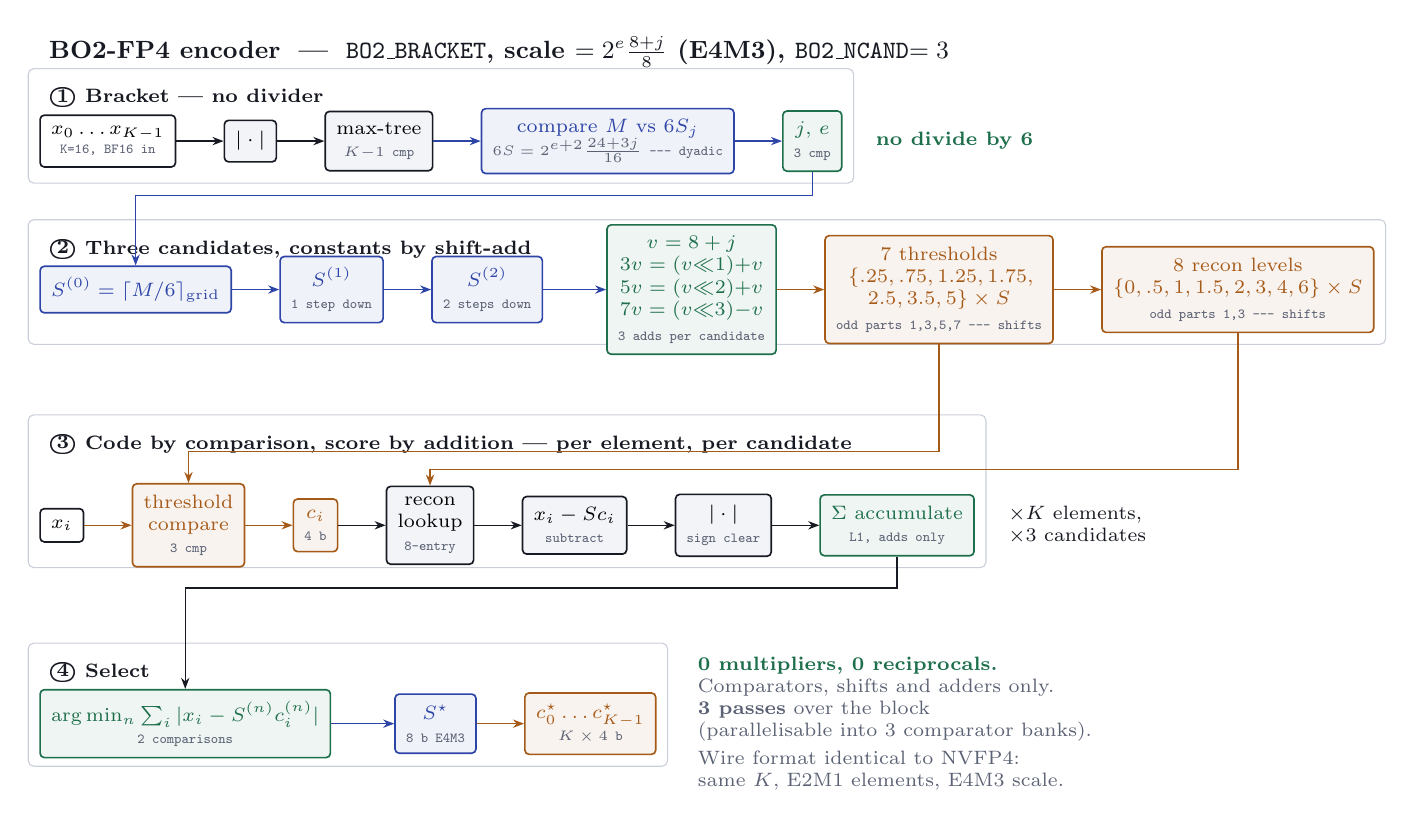
\begin{tikzpicture}[node distance=6mm]

\node[ttl] (t) {BO2-FP4 encoder \;---\; \texttt{BO2\_BRACKET}, scale $=2^{e}\tfrac{8+j}{8}$ (E4M3), \texttt{BO2\_NCAND}$=3$};

% ---------- stage 1: bracket, no divide ----------------------------------
\node[lbl,below=3.5mm of t.west,anchor=north west,font=\scriptsize\bfseries,text=inkc] (s1l)
  {\textcircled{1} Bracket --- no divider};
\node[blk,below=2mm of s1l.west,anchor=north west] (x) {$x_0\dots x_{K-1}$\\[-1pt]\dt{K=16, BF16 in}};
\node[op,right=of x]    (abs) {$|\cdot|$};
\node[op,right=of abs]  (max) {max-tree\\\dt{$K{-}1$ cmp}};
\node[scaleb,right=of max] (cmp6) {compare $M$ vs $6S_j$\\\dt{$6S=2^{e+2}\frac{24+3j}{16}$ --- dyadic}};
\node[free,right=of cmp6] (jsel) {$j$, $e$\\\dt{3 cmp}};
\draw[ar](x)--(abs); \draw[ar](abs)--(max); \draw[arS](max)--(cmp6); \draw[arS](cmp6)--(jsel);
\node[lbl,right=3mm of jsel,align=left,text=freec]
  {\textbf{no divide by 6}};

% ---------- stage 2: candidates + constants ------------------------------
\node[lbl,anchor=north west,font=\scriptsize\bfseries,text=inkc] (s2l)
  at ($(s1l.west|-x.south)+(0,-8mm)$)
  {\textcircled{2} Three candidates, constants by shift-add};
\node[scaleb,below=2mm of s2l.west,anchor=north west] (Sc) {$S^{(0)}=\lceil M/6\rceil_{\mathrm{grid}}$};
\node[scaleb,right=of Sc] (S1) {$S^{(1)}$\\\dt{1 step down}};
\node[scaleb,right=of S1] (S2) {$S^{(2)}$\\\dt{2 steps down}};
\draw[arS](jsel.south)--++(0,-3mm)-|(Sc.north);
\draw[arS](Sc)--(S1); \draw[arS](S1)--(S2);

\node[free,right=8mm of S2] (vconst) {$v=8+j$\\
  $3v=(v{\ll}1){+}v$\\ $5v=(v{\ll}2){+}v$\\ $7v=(v{\ll}3){-}v$\\[1pt]\dt{3 adds per candidate}};
\node[elemb,right=of vconst] (thr) {7 thresholds\\
  $\{.25,.75,1.25,1.75,\!$\\$2.5,3.5,5\}\times S$\\[1pt]\dt{odd parts 1,3,5,7 --- shifts}};
\node[elemb,right=of thr] (rec) {8 recon levels\\
  $\{0,.5,1,1.5,2,3,4,6\}\times S$\\[1pt]\dt{odd parts 1,3 --- shifts}};
\draw[arS](S2)--(vconst); \draw[arE](vconst)--(thr); \draw[arE](thr)--(rec);

% ---------- stage 3: per element, per candidate --------------------------
\node[lbl,anchor=north west,font=\scriptsize\bfseries,text=inkc] (s3l)
  at ($(s1l.west|-vconst.south)+(0,-9mm)$)
  {\textcircled{3} Code by comparison, score by addition --- per element, per candidate};
\node[blk,below=8mm of s3l.west,anchor=north west] (xi) {$x_i$};
\node[elemb,right=of xi] (tc) {threshold\\compare\\\dt{3 cmp}};
\node[elemb,right=of tc] (ci) {$c_i$\\\dt{4 b}};
\node[op,right=of ci]    (lu) {recon\\lookup\\\dt{8-entry}};
\node[op,right=of lu]    (sb) {$x_i-Sc_i$\\\dt{subtract}};
\node[op,right=of sb]    (ab) {$|\cdot|$\\\dt{sign clear}};
\node[free,right=of ab]  (ac) {$\Sigma$ accumulate\\\dt{L1, adds only}};
\node[lbl,right=3mm of ac,align=left,text=inkc,font=\scriptsize]
  {$\times K$ elements,\\$\times 3$ candidates};
\draw[arE](xi)--(tc); \draw[arE](tc)--(ci); \draw[ar](ci)--(lu);
\draw[ar](lu)--(sb); \draw[ar](sb)--(ab); \draw[ar](ab)--(ac);
\draw[arE](thr.south) |- ($(tc.north)+(0,4mm)$) -| (tc.north);
\draw[arE](rec.south) |- ($(lu.north)+(0,2mm)$) -| (lu.north);

% ---------- stage 4: select ----------------------------------------------
\node[lbl,anchor=north west,font=\scriptsize\bfseries,text=inkc] (s4l)
  at ($(s1l.west|-tc.south)+(0,-11mm)$)
  {\textcircled{4} Select};
\node[free,below=2mm of s4l.west,anchor=north west] (arg)
  {$\arg\min_{n} \sum_i |x_i - S^{(n)}c_i^{(n)}|$\\\dt{2 comparisons}};
\node[scaleb,right=8mm of arg] (sout) {$S^\star$\\\dt{8 b E4M3}};
\node[elemb,right=of sout] (cout) {$c_0^\star\dots c_{K-1}^\star$\\\dt{$K\times4$ b}};
\draw[ar](ac.south)--++(0,-4mm)-|(arg.north);
\draw[arS](arg)--(sout); \draw[arE](sout)--(cout);
\node[lbl,right=4mm of cout,align=left]
  {\textcolor{freec}{\textbf{0 multipliers, 0 reciprocals.}}\\
   Comparators, shifts and adders only.\\
   \textbf{3 passes} over the block\\
   (parallelisable into 3 comparator banks).\\[2pt]
   Wire format identical to NVFP4:\\
   same $K$, E2M1 elements, E4M3 scale.};

\begin{scope}[on background layer]
  \node[fit=(s1l)(jsel),draw=hairc,rounded corners=2pt,inner sep=4pt]{};
  \node[fit=(s2l)(rec),draw=hairc,rounded corners=2pt,inner sep=4pt]{};
  \node[fit=(s3l)(ac),draw=hairc,rounded corners=2pt,inner sep=4pt]{};
  \node[fit=(s4l)(cout),draw=hairc,rounded corners=2pt,inner sep=4pt]{};
\end{scope}
\end{tikzpicture}
\end{document}
